%                                                                 aa.dem
% AA vers. 9.1, LaTeX class for Astronomy & Astrophysics
% demonstration file
%                                                       (c) EDP Sciences
%-----------------------------------------------------------------------
%
%\documentclass[referee]{aa} % for a referee version
%\documentclass[onecolumn]{aa} % for a paper on 1 column  
%\documentclass[longauth]{aa} % for the long lists of affiliations 
%\documentclass[letter]{aa} % for the letters 
%\documentclass[bibyear]{aa} % if the references are not structured 
% according to the author-year natbib style


%
\documentclass[11pt]{aa}  
%%%%%%%%%%%%%%%%%%%%%%%%%%%%%%%%%%%%%%%%
\usepackage{graphicx} % Required for inserting images
\usepackage[french]{babel}
\usepackage[T1]{fontenc}
\selectlanguage{french}
\usepackage[utf8]{inputenc}
\usepackage{amsmath}
\usepackage{amsfonts,amsthm, amssymb}
\usepackage{esvect}
\usepackage{array}
%\usepackage[top=2cm,bottom=2cm,left=2cm,right=2cm]{geometry}
\graphicspath{./images/}
\usepackage{hyperref}
\usepackage{lipsum}
\usepackage{caption}  % Pour ajuster l'espacement des légendes
\usepackage{enumitem}
\usepackage{float} % pour forcer le positionnement des figures
\setlength{\textfloatsep}{0pt}  % Espace entre figure/table et texte
\setlength{\intextsep}{0pt}     % Espace au-dessus et au-dessous des flottants en ligne
\usepackage{siunitx}
\usepackage{titlesec}           %Personnaliser les espacement avant et après les titres et sous-titres


%%%%%%%%%%%%%%%%%%%%%%%%%%%%%%%%%%%%%%%%
%\usepackage[options]{hyperref}
% To add links in your PDF file, use the package "hyperref"
% with options according to your LaTeX or PDFLaTeX drivers.
%

% \abstract{}{}{}{}{} 
% 5 {} token are mandatory
 
  %\abstract
  % context heading (optional)
  % {} leave it empty if necessary  
  % aims heading (mandatory)
  % {}
  % methods heading (mandatory)
  % {}
  % results heading (mandatory)
  % {}
  % conclusions heading (optional), leave it empty if necessary 
  % {}


\title{Identification et simulation des observations d'objets du système solaire à l'aide de MICADO, instrument de première lumière qui sera monté sur le futur télescope géant de l'ESO}
\titlerunning{Simulation d'observations d'objets du système solaire à l'aide de MICADO}

\author{Antonin Pelletier
          }

\institute{L3 Magistère de Physique, Université Paris-Cité, France\\
         \email{antonin.pelletier@etu.u-paris.fr}
         }

\date{Date de dépôt: Vendredi 28 juin 2024}

\abstract {Mon stage s'est déroulé du 21/05/24 au 28/06/24 à l'observatoire de Paris, au sein du LESIA sous la tutelle de Frédéric Merlin}
   \keywords{ Objets Transneptuniens, Planétologie, Simulation, Photométrie astronomique
               }

%--------------------------------------------------------------------

\titlespacing*{\section}
{0pt}{*1}{*0.5}


\begin{document} 

\maketitle

\section{Introduction}
On nomme objets transneptuniens (OTNs) l'ensemble des corps se trouvant dans le système solaire au delà de l'orbite de Neptune et qui y restent en permanence. Les plus connus et massifs sont Pluton, auparavant classifié comme une planète et Eris. Leur étude est particulièrement intéressante car ce sont des objets qui n'ont presque pas évolué depuis la création du système solaire, ils sont donc d'importants vestiges du disque protoplanétaire et leur composition peut nous renseigner sur les éléments et les conditions présents il y a 4,5 milliards d'années.\\
L'Extremely Large Telescope (ELT) est un projet de télescope de l'observatoire européen austral (ESO) qui sera déployé à plus de 3000m d'altitude, au Cerro Armazones au Chili. Il aura un diamètre de 39,3m et sa première lumière est prévue pour 2028.\\ L'instrument auquel le LESIA contribue est la caméra optique à imagerie adaptative MICADO, prévue pour l'infrarouge proche, soit entre $0.8$ et $2.4\mu m$. Elle a été conçue pour fonctionner de paire avec l'optique adaptative (AO) de l'ELT \citep{ref_technique_MICADO}. Cette technique consiste à corriger en temps réel les déformations du front d'onde dues à l'atmosphère ainsi qu'à la traversée des éléments optiques du télescope. Plusieurs solutions existent pour améliorer les performances de MICADO dans le cadre de l'AO : utiliser une étoile de référence assez brillante qui se trouve dans le champ d'observation durant tout le temps de pose (c'est la méthode Single Conjuguate Adaptative Optics, que le LESIA est chargé de fournir) ou bien la création d'étoiles artificielles avec des LASERs dirigés vers le ciel. On peut également n'utiliser que la cible scientifique, à condition qu'elle soit assez petite (moins de 2 secondes d'arc de diamètre). In fine, l'objectif de l'AO est de se rapprocher au maximum des limites de diffraction de l'ELT.
\section{Objectifs du stage}
Le but de ce stage est de modéliser en langage python des objets du système solaire (principalement des OTNs) que l'on souhaite observer avec MICADO, puis de contraindre leurs propriétés physico-chimiques pour déterminer sous quelles conditions de temps d'exposition ou de magnitude des variations dans la chimie des objets seront détectables par l'ELT.

\section{Méthodologie}
Les OTNs simulés sont créés informatiquement en utilisant la bibliothèque python \textit{Scopesim} et sont composés de deux parties : une caractéristique spatiale, et une caractéristique spectrale. On utilisera ce découpage pour faire des variations dans la composition chimique de certaines parties de l'objet plus tard. Quand on "observe" un objet, il passe par le "train optique" de MICADO. Ce dernier réalise plusieurs étapes dont on détaillera une partie, il applique notamment la fonction d'étalement de point (PSF en anglais) qui rend compte de la déformation du front d'onde dans le cas d'un ciel moyen d'un point de vue statistique. Cela aboutit à une déformation de tout objet, même ponctuel, observé par un télescope sur un capteur CCD ou CMOS.\\

Plusieurs bibliothèques spécifiques à l'astrophysique m'ont été utiles durant ce stage :
\begin{itemize}
    
    \item[\textbullet] \textit{Scopesim} est l'outil principal utilisé car il s'agit d'un simulateur d'instruments astronomiques. Basé sur son prédécesseur \textit{SimCADO}, il m'a permis de simuler l'observation par MICADO des objets que j'ai créé. Ces objets, pour passer dans le train optique simulé de MICADO, doivent être du type \textit{Scopesim.Source} \citep{scopesim}.
    \item[\textbullet] \textit{Scopesim Templates} est un ensemble de fonctions facilitant la création d'objets \textit{Scopesim.Source} tels que des étoiles uniques, des champs d'étoiles ou des galaxies, le tout sur un ciel de fond qui dépend du temps d'exposition choisi. Après plusieurs tests j'ai pu mettre en évidence le fait que ce bruit de fond n'est pas aléatoire.
    \item[\textbullet] \textit{Spextra} fait partie de la suite de bibliothèques affiliées à \textit{Scopesim} et apporte une interface python à la plupart des bibliothèques spectrales de la communauté. Je l'ai également utilisée pour créer les spectres qu'on obtiendrait en observant les OTNs Pluton, Charon, Eris et 2005RR43.  
    %générer des filtres afin de renormaliser des spectres en réflectance sur des bandes de longueur d'onde données.
    \item[\textbullet] \textit{Pyckles}, faisant également partie de l'environnement \textit{Scopesim}, permet un accès simplifié au catalogue des types spectraux Pyckles et Brown, que j'ai utilisés pour récupérer le spectre d'une étoile G2V de type solaire.
    %\item[\textbullet] \textit{Synphot} est une bibliothèque permettant de traiter efficacement des spectres et des filtres, je l'ai utilisée en complément de \textit{Spextra} et \textit{Pyckles} pour des fonctions spécifiques \citep{synphot}.
\end{itemize}




Afin de pouvoir comparer des résultats, j'ai élaboré une fonction prenant en argument les caractéristiques physico-chimiques de l'objet à étudier et qui renvoie la simulation d'observation par MICADO d'un tel objet.

On commence par créer une grille de 1024x1024 pixels pour y placer notre objet. Chaque pixel sur MICADO fait 4mas de côté et le champ de vue total est de 50"x50". \\Quand on observe un OTN, c'est la lumière réfléchie du Soleil qui nous parvient. Or les objets étudiés ici sont résolus (i.e non ponctuels sur le détecteur), on ajoute donc sur notre grille la contrainte que le flux de l'objet doit respecter la loi de Lambert :
\begin{equation}
    I = I_0.cos(\theta)
\end{equation}
où $I$ est l'intensité perçue par l'observateur, $I_0$ l'intensité de la source, ici le Soleil. $\theta$ est l'angle compté à partir du point subsolaire, c'est à dire le point sur l'objet où le Soleil est observé au zénith. Dans le cadre des OTNs, l'angle de phase est souvent très faible, ce qui implique que de notre point de vue le "bord" de l'objet soit moins brillant que son centre (voir sur la Fig.\ref{fig:fig1}). \\
On réalise également un suréchantillonnage pour que les bords des objets étendus soient rendus correctement. Cela consiste à diviser chaque pixel en une nouvelle grille de 9x9 sous-pixels et à calculer la distance au centre de l'objet $d$ pour chaque sous-pixel. Tous ceux qui respectent la condition $d \leq r$ avec $r$ le rayon de l'OTN sont comptabilisés comme faisant partie de l'objet. Une fois cette opération effectuée sur toute l'image, on regroupe chaque grille de 9x9 à nouveau en un pixel unique, dont la valeur est la fraction des sous-pixels le composant faisant partie de l'objet. Par exemple un pixel dont 27 sous-pixels sur 81 respectent la condition $d \leq r$ aura pour valeur $\frac{1}{3}$. \\ A ce moment là chaque pixel contient une fraction correspondant à la quantité de flux que l'on doit lui assigner.  \\
 On peut alors convertir la magnitude totale en flux que l’on répartit suivant la distribution de flux précédemment déterminée.\\
On rajoute ensuite un bruit de mesure aléatoire sur le flux de chaque pixel, qui représente ce que l'on peut obtenir lors d'observations en conditions réelles. Ce bruit dépend du rapport $\frac{signal}{bruit}$, aussi appelé SNR, qui est calculé à partir du flux (et donc de la magnitude), du temps de pose voulu et d'un SNR de référence \citep{SNR}. \\On peut désormais convertir les flux "partiels" en "magnitudes partielles" puis convertir chacun des pixels de l'image en autant d'objets \textit{Scopesim.Source} via le package \textit{scopesim template}. Chaque pixel peut avoir un spectre différent, ce qui aura un intérêt dans la prochaine partie.\\
Maintenant que l'objet étendu est créé, on peut l'observer en utilisant le train optique de MICADO. On récupère alors les cartes de flux issues de ces observations, qui sont déformées par la PSF ( image de droite sur la Fig.\ref{fig:fig1}). On constate alors que si l'objet "idéal" de la première image était bien restreint au diamètre d'Éris, une fois observé par MICADO l'objet "s'étale" en dehors du cercle tracé.
%fig1 avant

\section{Résultats obtenus}
%Les paramètres importants sur lesquels on peut jouer sont le diam
L'idée derrière cette simulation est de pouvoir faire varier certains pixels des objets générés pour représenter la présence d'éléments chimiques connus comme étant présents à la surface des OTNs et ayant des bandes d'absorption caractéristiques : 
\begin{itemize}
    \item[\textbullet] La présence de carbone sur un objet induit une réduction de l'albédo, directement visible lors de l'observation, par exemple dans un filtre J ($1.1-1.4 \mu m$).
    \item[\textbullet] Les glaces d'eau $H_2O$ et de méthane $CH_4$ ont des pics d'absorbance caractéristiques : $1.65\mu m$ et $2.3 \mu m$ pour la glace de méthane, $1.5 \mu m$ et $2 \mu m$ pour la glace d'eau \citep{these_merlin}.
\end{itemize}

Si les variations d'albedo sont valables dans toutes les longeurs d'ondes, ce n'est pas le cas des variations en terme de glace d'$H_2O$ et de $CH_4$. La technique utilisée consiste alors à observer le même objet dans deux filtres distincts ; un premier pour lequel les bandes d'absorption ne sont pas visibles, et un second pour lequel c'est le cas.\\ Par exemple en choisissant les filtres J et H ($1.5-1.8\mu m$) puis en soustrayant l'un à l'autre, il est possible de mettre en évidence le pic d'absorption à $1.65 \mu m$ de la glace d'eau et celui à $1.5 \mu m$ de la glace de méthane.
%anciennement fig2
On applique donc sur l'ensemble de l'objet un spectre de type G2V (i.e solaire) multiplié à un spectre en réflectance contenant une certaine proportion de glace de $CH_4$ et de glace d'$H_2O$. Sur une zone de l'objet (un "patch"), constituée de un à plusieurs pixels, on modifie la proportion des espèces chimiques supposées présentes avant d’observer cet effet selon la méthode exposée ci-dessus. \\ On peut alors déterminer si MICADO sera capable de détecter une telle variation au delà du bruit de mesure. La trentaine de filtres disponibles sur MICADO \citep{carac_tech_et_prez} permettra de cibler précisément certaines longueurs d'ondes et les molécules associées.\\
Je propose ici un exemple concret d'utilisation de ma fonction. Deux spectres sont donnés sur la Fig.\ref{fig:fig2}. On peut voir qu'à $1.62\mu m$ (on rappelle que $1 \mu m = 10000 \text{\AA}$) il y a une différence de réflectance de près de 20\% entre les deux spectres alors qu'elle est à peine de 0.3\% à $2.1\mu m$. On peut alors choisir les filtres H-short (centré sur $1.59\mu m$) et K-mid (centré sur $2.1\mu m$) de MICADO pour mettre en évidence un patch de 4x4 pixels ajouté en bas à gauche d'un hypothétique OTN dont toute la surface correspondrait au premier spectre (10\% $H_2O$/90\% $CH_4$) à l'exception d'une portion dont la chimie serait plutôt celle du second spectre (50\% $H_2O$/50\% $CH_4$). Le résultat est présenté dans la Fig.\ref{fig:fig3} et l'on voit en effet que le patch apparaît plus lumineux lorsque l'on soustrait les observations faites avec les filtres H-short et K-mid. Afin de mettre en évidence visuellement la différence j'ai retiré le bruit de mesure, qui normalement est pris en compte pour les cibles scientifiques.\\ Il ne s'agit là que d'un cas de figure spécifique avec un objet de diamètre semblable à Eris, mais la fonction développée permet de répondre à différentes problématiques en modifiant les paramètres suivants : la magnitude, les dimensions (l'objet peut être une ellipse), le profil (uniforme ou lambertien), le temps d'exposition $T_{exp}$, le filtre utilisé pour la normalisation à la création de l'objet, le filtre utilisé pour l'observation, le spectre de l'objet, le spectre du patch et la taille de chaque pixel.
%anciennement fig3 ici
%Regarde la big fonction, tout ce qui est dedans est le résultat d'1 mois d'efforts. La décortiquer intégralement te fait ta partie (objets (profils, mags, formes), spectres, filtres, sources)
\section{Conclusion}
\vspace{-0.5em}
Durant mon stage au LESIA, j'ai développé un ensemble d'outils pour créer des objets \textit{Scopesim}, traiter leur composantes spectrales et spatiales pour correspondre aux contraintes physiques des objets étudiés au sein du système solaire telles qu'un profil lambertien ou du bruit de mesure. J'ai également pu établir des résultats sur les temps de pose souhaités dans le cas d'Éris.\\
L'étape suivante est de faire varier différents paramètres, tels que le diamètre ou la magnitude de l'objet étudié, pour pouvoir calculer le temps d'exposition nécessaire pour détecter une variation physico-chimique de la surface donnée. On pourra ainsi déterminer le seuil de détection en fonction de $T_{exp}$ et de la magnitude pour un objet fixé. Cela peut ensuite s'étendre à tous les OTNs (résolus de préférence) que l'ELT pourra observer et dont on connaît déjà la composition globale. Contraindre des paramètres de cette façon permettrait d'anticiper plus efficacement les observations qui seront faites avec MICADO lors de la première lumière de l'instrument, à l'horizon 2029.
%La fonction que j'ai développé et l'ensemble des sous-fonctions qui lui sont associées seront utiles pour déterminer l'observabilité de variations spécifiques de composition chimique à la surface des OTNs qui seront résolus avec MICADO sur l'ELT. \\ Une autre part importante du travail restant à accomplir concerne la spectroscopie infrarouge : trois fentes (de 16mas x 3", 20mas x 15" et 48 mas x 3") sont prévues sur l'instrument pour l'étude d'objets compacts, tels que les OTNs. Grâce à la spectroscopie on pourra confirmer ou infirmer la présence de certaines molécules sur la surface des OTNs ciblés par l'ELT. Les performances de MICADO dans le cadre de la SCAO sont grandement dépendantes de la magnitude de l'étoile ciblée : au dela de 15

%\newpage
\begin{figure}[H]
    \centering
    
\includegraphics[width=0.5\textwidth]{Images/comparaison_avant_apres_train_optique.png}
    \caption{Carte de flux d'Eris avant et après passage dans le train optique de MICADO. Pour la première image seulement les pixels blancs valent 0 mais le cercle rouge est le périmètre d'Éris dans les deux cas.}
    \label{fig:fig1} % Label pour référencer la figure
\end{figure}
\begin{figure}[H]
    \centering
    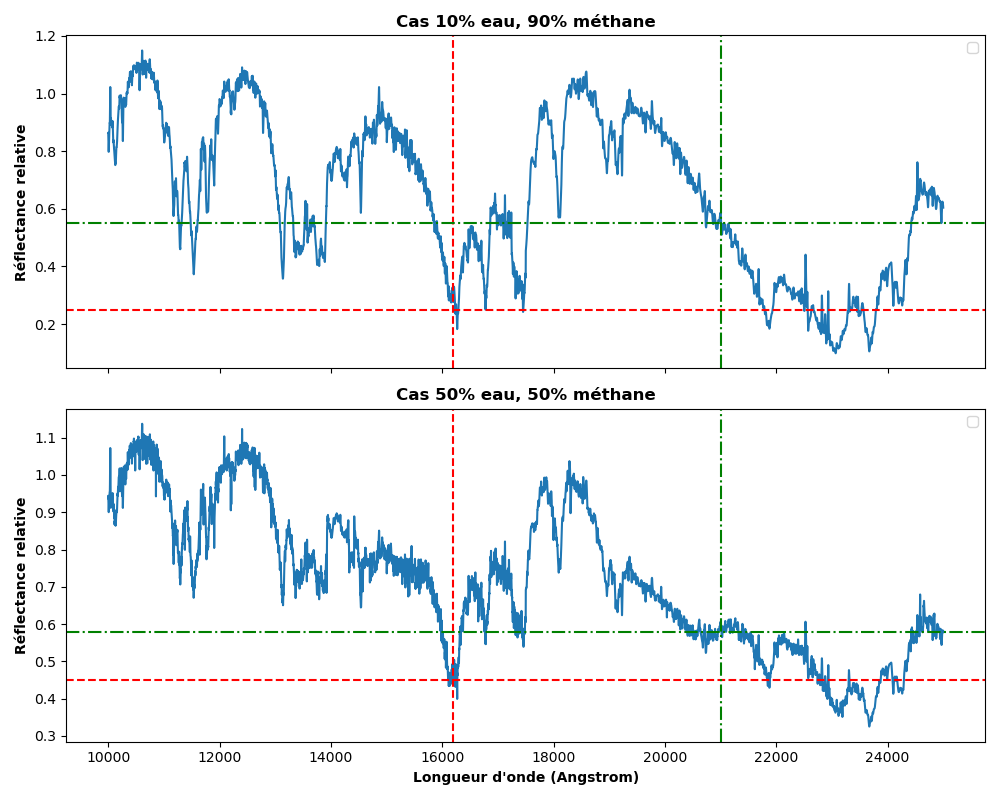
\includegraphics[width=0.5\textwidth]{Images/2_spectres_no_grid.png}
    \caption{Exemple de spectres en réflectance dont on a modifié la composition.}
    \label{fig:fig2} % Label pour référencer la figure
\end{figure}
\begin{figure}[H]
    \centering
    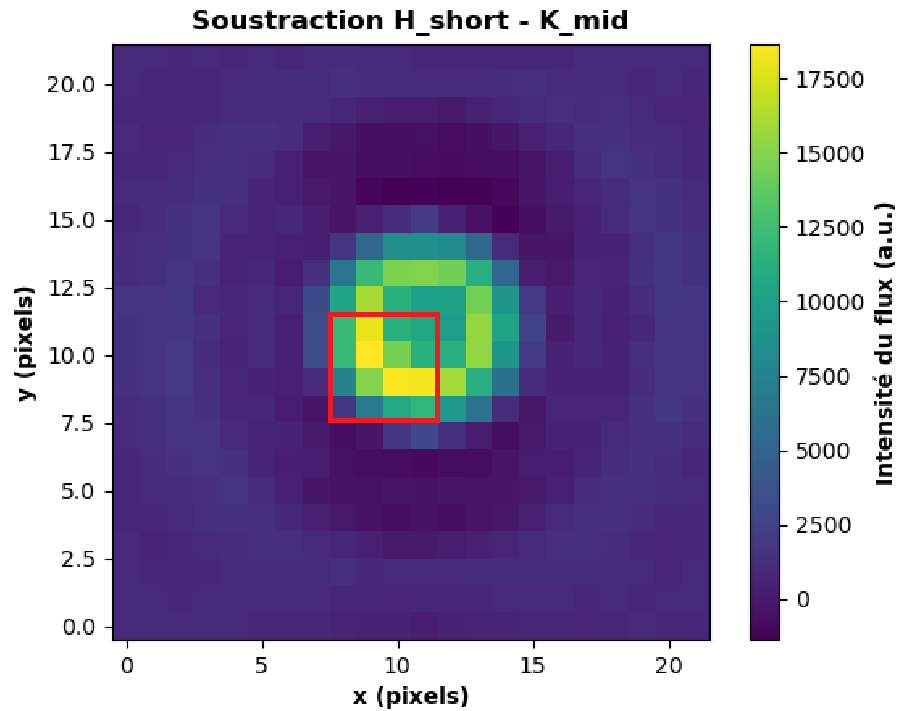
\includegraphics[width=0.5\textwidth]{Images/soustraction.png}
    \caption{Carte de flux comparant le même objet observé dans deux filtres différents, le patch est encadré en rouge.}
    \label{fig:fig3} % Label pour référencer la figure
\end{figure}
    

%\nocite{*}
\bibliographystyle{aa}
\bibliography{biblio.bib}

\end{document}
% ================= ANNEXE ==================== %




%
%%%%%%%%%%%%%%%%%%%%%%%%%%%%%%%%%%%%%%%%%%%%%%%%%%%%%%%%%%%%%%
Example below of non-structurated natbib references  
To use the v8.3 macros with this form of composition of bibliography, 
the option "bibyear" should be added to the command line 
"\documentclass[bibyear]{aa}".
%%%%%%%%%%%%%%%%%%%%%%%%%%%%%%%%%%%%%%%%%%%%%%%%%%%%%%%%%%%%%%
%Je suis quelqu'un d'extrêmement talentueux d'ailleurs, et beau. Très beau. (Cf Garance)
\begin{thebibliography}{}

  \bibitem[1966]{baker} Baker, N. 1966,
      in Stellar Evolution,
      ed.\ R. F. Stein,\& A. G. W. Cameron
      (Plenum, New York) 333

   \bibitem[1988]{balluch} Balluch, M. 1988,
      A\&A, 200, 58

   \bibitem[1980]{cox} Cox, J. P. 1980,
      Theory of Stellar Pulsation
      (Princeton University Press, Princeton) 165

   \bibitem[1969]{cox69} Cox, A. N.,\& Stewart, J. N. 1969,
      Academia Nauk, Scientific Information 15, 1

   \bibitem[1980]{mizuno} Mizuno H. 1980,
      Prog. Theor. Phys., 64, 544
   
   \bibitem[1987]{tscharnuter} Tscharnuter W. M. 1987,
      A\&A, 188, 55
  
   \bibitem[1992]{terlevich} Terlevich, R. 1992, in ASP Conf. Ser. 31, 
      Relationships between Active Galactic Nuclei and Starburst Galaxies, 
      ed. A. V. Filippenko, 13

   \bibitem[1980a]{yorke80a} Yorke, H. W. 1980a,
      A\&A, 86, 286

   \bibitem[1997]{zheng} Zheng, W., Davidsen, A. F., Tytler, D. \& Kriss, G. A.
      1997, preprint
\end{thebibliography}
%
%%%%%%%%%%%%%%%%%%%%%%%%%%%%%%%%%%%%%%%%%%%%%%%%%%%%%%%%%%%%%%
Examples for figures using graphicx
A guide "Using Imported Graphics in LaTeX2e"  (Keith Reckdahl)
is available on a lot of LaTeX public servers or ctan mirrors.
The file is : epslatex.pdf 
%%%%%%%%%%%%%%%%%%%%%%%%%%%%%%%%%%%%%%%%%%%%%%%%%%%%%%%%%%%%%%

%-------------------------------------------------------------
%                 A figure as large as the width of the column
%-------------------------------------------------------------
   \begin{figure}
   \centering
   \includegraphics[width=\hsize]{empty.eps}
      \caption{Vibrational stability equation of state
               $S_{\mathrm{vib}}(\lg e, \lg \rho)$.
               $>0$ means vibrational stability.
              }
         \label{FigVibStab}
   \end{figure}
%
%-------------------------------------------------------------
%                                    One column rotated figure
%-------------------------------------------------------------
   \begin{figure}
   \centering
   \includegraphics[angle=-90,width=3cm]{empty.eps}
      \caption{Vibrational stability equation of state
               $S_{\mathrm{vib}}(\lg e, \lg \rho)$.
               $>0$ means vibrational stability.
              }
         \label{FigVibStab}
   \end{figure}
%
%-------------------------------------------------------------
%                        Figure with caption on the right side 
%-------------------------------------------------------------
   \begin{figure}
   \sidecaption
   \includegraphics[width=3cm]{empty.eps}
      \caption{Vibrational stability equation of state
               $S_{\mathrm{vib}}(\lg e, \lg \rho)$.
               $>0$ means vibrational stability.
              }
         \label{FigVibStab}
   \end{figure}
%
%-------------------------------------------------------------
%                                Figure with a new BoundingBox 
%-------------------------------------------------------------
   \begin{figure}
   \centering
   \includegraphics[bb=10 20 100 300,width=3cm,clip]{empty.eps}
      \caption{Vibrational stability equation of state
               $S_{\mathrm{vib}}(\lg e, \lg \rho)$.
               $>0$ means vibrational stability.
              }
         \label{FigVibStab}
   \end{figure}
%
%-------------------------------------------------------------
%                                      The "resizebox" command 
%-------------------------------------------------------------
   \begin{figure}
   \resizebox{\hsize}{!}
            {\includegraphics[bb=10 20 100 300,clip]{empty.eps}
      \caption{Vibrational stability equation of state
               $S_{\mathrm{vib}}(\lg e, \lg \rho)$.
               $>0$ means vibrational stability.
              }
         \label{FigVibStab}
   \end{figure}
%
%-------------------------------------------------------------
%                                             Two column Figure 
%-------------------------------------------------------------
   \begin{figure*}
   \resizebox{\hsize}{!}
            {\includegraphics[bb=10 20 100 300,clip]{empty.eps}
      \caption{Vibrational stability equation of state
               $S_{\mathrm{vib}}(\lg e, \lg \rho)$.
               $>0$ means vibrational stability.
              }
         \label{FigVibStab}
   \end{figure*}
%
%-------------------------------------------------------------
%                                             Simple A&A Table
%-------------------------------------------------------------
%
\begin{table}
\caption{Nonlinear Model Results}             % title of Table
\label{table:1}      % is used to refer this table in the text
\centering                          % used for centering table
\begin{tabular}{c c c c}        % centered columns (4 columns)
\hline\hline                 % inserts double horizontal lines
HJD & $E$ & Method\#2 & Method\#3 \\    % table heading 
\hline                        % inserts single horizontal line
   1 & 50 & $-837$ & 970 \\      % inserting body of the table
   2 & 47 & 877    & 230 \\
   3 & 31 & 25     & 415 \\
   4 & 35 & 144    & 2356 \\
   5 & 45 & 300    & 556 \\ 
\hline                                   %inserts single line
\end{tabular}
\end{table}
%
%-------------------------------------------------------------
%                                             Two column Table 
%-------------------------------------------------------------
%
\begin{table*}
\caption{Nonlinear Model Results}             
\label{table:1}      
\centering          
\begin{tabular}{c c c c l l l }     % 7 columns 
\hline\hline       
                      % To combine 4 columns into a single one 
HJD & $E$ & Method\#2 & \multicolumn{4}{c}{Method\#3}\\ 
\hline                    
   1 & 50 & $-837$ & 970 & 65 & 67 & 78\\  
   2 & 47 & 877    & 230 & 567& 55 & 78\\
   3 & 31 & 25     & 415 & 567& 55 & 78\\
   4 & 35 & 144    & 2356& 567& 55 & 78 \\
   5 & 45 & 300    & 556 & 567& 55 & 78\\
\hline                  
\end{tabular}
\end{table*}
%
%-------------------------------------------------------------
%                                          Table with notes 
%-------------------------------------------------------------
%
% A single note
\begin{table}
\caption{\label{t7}Spectral types and photometry for stars in the
  region.}
\centering
\begin{tabular}{lccc}
\hline\hline
Star&Spectral type&RA(J2000)&Dec(J2000)\\
\hline
69           &B1\,V     &09 15 54.046 & $-$50 00 26.67\\
49           &B0.7\,V   &*09 15 54.570& $-$50 00 03.90\\
LS~1267~(86) &O8\,V     &09 15 52.787&11.07\\
24.6         &7.58      &1.37 &0.20\\
\hline
LS~1262      &B0\,V     &09 15 05.17&11.17\\
MO 2-119     &B0.5\,V   &09 15 33.7 &11.74\\
LS~1269      &O8.5\,V   &09 15 56.60&10.85\\
\hline
\end{tabular}
\tablefoot{The top panel shows likely members of Pismis~11. The second
panel contains likely members of Alicante~5. The bottom panel
displays stars outside the clusters.}
\end{table}
%
% More notes
%
\begin{table}
\caption{\label{t7}Spectral types and photometry for stars in the
  region.}
\centering
\begin{tabular}{lccc}
\hline\hline
Star&Spectral type&RA(J2000)&Dec(J2000)\\
\hline
69           &B1\,V     &09 15 54.046 & $-$50 00 26.67\\
49           &B0.7\,V   &*09 15 54.570& $-$50 00 03.90\\
LS~1267~(86) &O8\,V     &09 15 52.787&11.07\tablefootmark{a}\\
24.6         &7.58\tablefootmark{1}&1.37\tablefootmark{a}   &0.20\tablefootmark{a}\\
\hline
LS~1262      &B0\,V     &09 15 05.17&11.17\tablefootmark{b}\\
MO 2-119     &B0.5\,V   &09 15 33.7 &11.74\tablefootmark{c}\\
LS~1269      &O8.5\,V   &09 15 56.60&10.85\tablefootmark{d}\\
\hline
\end{tabular}
\tablefoot{The top panel shows likely members of Pismis~11. The second
panel contains likely members of Alicante~5. The bottom panel
displays stars outside the clusters.\\
\tablefoottext{a}{Photometry for MF13, LS~1267 and HD~80077 from
Dupont et al.}
\tablefoottext{b}{Photometry for LS~1262, LS~1269 from
Durand et al.}
\tablefoottext{c}{Photometry for MO2-119 from
Mathieu et al.}
}
\end{table}
%
%-------------------------------------------------------------
%                                       Table with references 
%-------------------------------------------------------------
%
\begin{table*}[h]
 \caption[]{\label{nearbylistaa2}List of nearby SNe used in this work.}
\begin{tabular}{lccc}
 \hline \hline
  SN name &
  Epoch &
 Bands &
  References \\
 &
  (with respect to $B$ maximum) &
 &
 \\ \hline
1981B   & 0 & {\it UBV} & 1\\
1986G   &  $-$3, $-$1, 0, 1, 2 & {\it BV}  & 2\\
1989B   & $-$5, $-$1, 0, 3, 5 & {\it UBVRI}  & 3, 4\\
1990N   & 2, 7 & {\it UBVRI}  & 5\\
1991M   & 3 & {\it VRI}  & 6\\
\hline
\noalign{\smallskip}
\multicolumn{4}{c}{ SNe 91bg-like} \\
\noalign{\smallskip}
\hline
1991bg   & 1, 2 & {\it BVRI}  & 7\\
1999by   & $-$5, $-$4, $-$3, 3, 4, 5 & {\it UBVRI}  & 8\\
\hline
\noalign{\smallskip}
\multicolumn{4}{c}{ SNe 91T-like} \\
\noalign{\smallskip}
\hline
1991T   & $-$3, 0 & {\it UBVRI}  &  9, 10\\
2000cx  & $-$3, $-$2, 0, 1, 5 & {\it UBVRI}  & 11\\ %
\hline
\end{tabular}
\tablebib{(1)~\citet{branch83};
(2) \citet{phillips87}; (3) \citet{barbon90}; (4) \citet{wells94};
(5) \citet{mazzali93}; (6) \citet{gomez98}; (7) \citet{kirshner93};
(8) \citet{patat96}; (9) \citet{salvo01}; (10) \citet{branch03};
(11) \citet{jha99}.
}
\end{table*}
%-------------------------------------------------------------
%                      A rotated Two column Table in landscape  
%-------------------------------------------------------------
\begin{sidewaystable*}
\caption{Summary for ISOCAM sources with mid-IR excess 
(YSO candidates).}\label{YSOtable}
\centering
\begin{tabular}{crrlcl} 
\hline\hline             
ISO-L1551 & $F_{6.7}$~[mJy] & $\alpha_{6.7-14.3}$ 
& YSO type$^{d}$ & Status & Comments\\
\hline
  \multicolumn{6}{c}{\it New YSO candidates}\\ % To combine 6 columns into a single one
\hline
  1 & 1.56 $\pm$ 0.47 & --    & Class II$^{c}$ & New & Mid\\
  2 & 0.79:           & 0.97: & Class II ?     & New & \\
  3 & 4.95 $\pm$ 0.68 & 3.18  & Class II / III & New & \\
  5 & 1.44 $\pm$ 0.33 & 1.88  & Class II       & New & \\
\hline
  \multicolumn{6}{c}{\it Previously known YSOs} \\
\hline
  61 & 0.89 $\pm$ 0.58 & 1.77 & Class I & \object{HH 30} & Circumstellar disk\\
  96 & 38.34 $\pm$ 0.71 & 37.5& Class II& MHO 5          & Spectral type\\
\hline
\end{tabular}
\end{sidewaystable*}
%-------------------------------------------------------------
%                      A rotated One column Table in landscape  
%-------------------------------------------------------------
\begin{sidewaystable}
\caption{Summary for ISOCAM sources with mid-IR excess 
(YSO candidates).}\label{YSOtable}
\centering
\begin{tabular}{crrlcl} 
\hline\hline             
ISO-L1551 & $F_{6.7}$~[mJy] & $\alpha_{6.7-14.3}$ 
& YSO type$^{d}$ & Status & Comments\\
\hline
  \multicolumn{6}{c}{\it New YSO candidates}\\ % To combine 6 columns into a single one
\hline
  1 & 1.56 $\pm$ 0.47 & --    & Class II$^{c}$ & New & Mid\\
  2 & 0.79:           & 0.97: & Class II ?     & New & \\
  3 & 4.95 $\pm$ 0.68 & 3.18  & Class II / III & New & \\
  5 & 1.44 $\pm$ 0.33 & 1.88  & Class II       & New & \\
\hline
  \multicolumn{6}{c}{\it Previously known YSOs} \\
\hline
  61 & 0.89 $\pm$ 0.58 & 1.77 & Class I & \object{HH 30} & Circumstellar disk\\
  96 & 38.34 $\pm$ 0.71 & 37.5& Class II& MHO 5          & Spectral type\\
\hline
\end{tabular}
\end{sidewaystable}
%
%-------------------------------------------------------------
%                              Table longer than a single page  
%-------------------------------------------------------------
% All long tables will be placed automatically at the end of the document
%
\longtab{
\begin{longtable}{lllrrr}
\caption{\label{kstars} Sample stars with absolute magnitude}\\
\hline\hline
Catalogue& $M_{V}$ & Spectral & Distance & Mode & Count Rate \\
\hline
\endfirsthead
\caption{continued.}\\
\hline\hline
Catalogue& $M_{V}$ & Spectral & Distance & Mode & Count Rate \\
\hline
\endhead
\hline
\endfoot
%%
Gl 33    & 6.37 & K2 V & 7.46 & S & 0.043170\\
Gl 66AB  & 6.26 & K2 V & 8.15 & S & 0.260478\\
Gl 68    & 5.87 & K1 V & 7.47 & P & 0.026610\\
         &      &      &      & H & 0.008686\\
Gl 86 
\footnote{Source not included in the HRI catalog. See Sect.~5.4.2 for details.}
         & 5.92 & K0 V & 10.91& S & 0.058230\\
\end{longtable}
}
%
%-------------------------------------------------------------
%                              Table longer than a single page
%                                            and in landscape, 
%                    in the preamble, use: \usepackage{lscape}
%-------------------------------------------------------------

% All long tables will be placed automatically at the end of the document
%
\longtab{
\begin{landscape}
\begin{longtable}{lllrrr}
\caption{\label{kstars} Sample stars with absolute magnitude}\\
\hline\hline
Catalogue& $M_{V}$ & Spectral & Distance & Mode & Count Rate \\
\hline
\endfirsthead
\caption{continued.}\\
\hline\hline
Catalogue& $M_{V}$ & Spectral & Distance & Mode & Count Rate \\
\hline
\endhead
\hline
\endfoot
%%
Gl 33    & 6.37 & K2 V & 7.46 & S & 0.043170\\
Gl 66AB  & 6.26 & K2 V & 8.15 & S & 0.260478\\
Gl 68    & 5.87 & K1 V & 7.47 & P & 0.026610\\
         &      &      &      & H & 0.008686\\
Gl 86
\footnote{Source not included in the HRI catalog. See Sect.~5.4.2 for details.}
         & 5.92 & K0 V & 10.91& S & 0.058230\\
\end{longtable}
\end{landscape}
}
%
%-------------------------------------------------------------
%               Appendices have to be placed at the end, after
%                                        \end{thebibliography}
%-------------------------------------------------------------
\end{thebibliography}

\begin{appendix} %First appendix
\section{Background galaxy number counts and shear noise-levels}
Because the optical images used in this analysis...
\begin{figure*}%f1
\includegraphics[width=10.9cm]{1787f23.eps}
\caption{Shown in greyscale is a...}
\label{cl12301}
\end{figure*}

In this case....
\begin{figure*}
\centering
\includegraphics[width=16.4cm,clip]{1787f24.ps}
\caption{Plotted above...}
\label{appfig}
\end{figure*}

Because the optical images...

\section{Title of Second appendix.....} %Second appendix
These studies, however, have faced...
\begin{table}
\caption{Complexes characterisation.}\label{starbursts}
\centering
\begin{tabular}{lccc}
\hline \hline
Complex & $F_{60}$ & 8.6 &  No. of  \\
...
\hline
\end{tabular}
\end{table}

The second method produces...
\end{appendix}
%
%
\end{document}

%
%-------------------------------------------------------------
%          For the appendices, table longer than a single page
%-------------------------------------------------------------

% Table will be print automatically at the end of the document, 
% after the whole appendices

\begin{appendix} %First appendix
\section{Background galaxy number counts and shear noise-levels}

% In the appendices do not forget to put the counter of the table 
% as an option

\longtab[1]{
\begin{longtable}{lrcrrrrrrrrl}
\caption{Line data and abundances ...}\\
\hline
\hline
Def & mol & Ion & $\lambda$ & $\chi$ & $\log gf$ & N & e &  rad & $\delta$ & $\delta$ 
red & References \\
\hline
\endfirsthead
\caption{Continued.} \\
\hline
Def & mol & Ion & $\lambda$ & $\chi$ & $\log gf$ & B & C &  rad & $\delta$ & $\delta$ 
red & References \\
\hline
\endhead
\hline
\endfoot
\hline
\endlastfoot
A & CH & 1 &3638 & 0.002 & $-$2.551 &  &  &  & $-$150 & 150 &  Jorgensen et al. (1996) \\                    
\end{longtable}
}% End longtab
\end{appendix}

%-------------------------------------------------------------
%                   For appendices and landscape, large table:
%                    in the preamble, use: \usepackage{lscape}
%-------------------------------------------------------------

\begin{appendix} %First appendix
%
\longtab[1]{
\begin{landscape}
\begin{longtable}{lrcrrrrrrrrl}
...
\end{longtable}
\end{landscape}
}% End longtab
\end{appendix}

%%%% End of aa.dem
